\documentclass[a4paper,10pt]{report}
\usepackage[french]{babel}
\usepackage[T1]{fontenc}
\usepackage[utf8]{inputenc}
\usepackage[left=2.5cm,top=2cm,right=2.5cm,nohead,nofoot]{geometry}
\usepackage{url}
\usepackage{graphicx}
\usepackage{float}
\usepackage[colorinlistoftodos]{todonotes}
\usepackage{mathtools}
\usepackage{listings}

\linespread{1.1}

\title{Les ombres au sein des jeux et des animations}
\begin{document}

% Super commande 
\newcommand*{\captionsource}[2]{%
  \caption[{#1}]{%
    #1%
    \\\hspace{\linewidth}%
    \textbf{Source:} #2%
  }%
}


% ___ PAGE DE GARDE ____

\begin{titlepage}
\begin{center}
\textbf{\textsc{UNIVERSIT\'E LIBRE DE BRUXELLES}}\\
\textbf{\textsc{Faculté des Sciences}}\\
\textbf{\textsc{Département d'Informatique}}
\vfill{}\vfill{}
\begin{center}{\Huge Les ombres au sein des jeux et des animations}\end{center}{\Huge \par}
\begin{center}{\large Bruno Rocha Pereira\\ Pierre Gérard\\ Antoine Carpentier}\end{center}{\Huge \par}
\vfill{}\vfill{}
\begin{flushleft}{\large \textbf{Superviseurs :}}\hfill{Tom Lenaerts et Jean-Sébastien Lerat}\end{flushleft}{\large\par}
\vfill{}\vfill{}\enlargethispage{3cm}
\textbf{Année académique 2014~-~2015}
\end{center}
\end{titlepage}

\begin{abstract}
Ce rapport présente les différentes techniques de rendu d'ombre par ordinateurs, les résultats obtenues lors l'implémentation et les perspectives de ces dernières.
\end{abstract}



\tableofcontents


\chapter{Introduction}

Une ombre est une ``zone sombre résultant de l'interception de la lumière ou de l'absence de lumière``\footnote{http://www.larousse.fr/dictionnaires/francais/ombre/55933}. C'est un élément indispensable au réalisme d'une scène d'animation ou de jeu vidéo. En effet ce sont les ombres qui vont apporter l'information quand à la position relative et à la taille des objets qui créent l'ombre. Dans le cas d'objets complexes, elles permettent d'obtenir des informations sur la forme des objets.
Dans le monde réel, on est souvent confronté à plusieurs sources lumineuses qui apportent chacune leur lot d'informations en plus.


Nous avons, lors de ce projet d'année, étudié l'impact des ombres sur le réalisme des animations et des jeux vidéos. Cette étude a été réalisée en utilisant et comparant différents algorithmes de génération d'ombre, plus ou moins réalistes.


Nous nous sommes intéressés plus particulièrement aux algorithmes en temps réel car ceux-ci sont plus intéressants et plus attractifs pour une présentation pour le Printemps des Sciences\footnote{http://www.printempsdessciences.be}.

Deux types d'ombres peuvent être distingués : les \textit{soft shadows} et les \textit{hard shadows}. Les premières ont des bords diffus et les secondes ont des bords nets. Plus la source de lumière est proche d'un objet, plus les bords d'une ombre réaliste sont diffus et inversément.
Dans ce projet, nous nous somme intéressé uniquement aux algorithmes de génération des \textit{soft shadows} car ils permettent également de générer des \textit{hard shadows}.

Nous avons testé les différents aspects et effets des ombres dans différents scénarios que nous avons mis en application. Nous avons fait varier les objets, les sources lumineuses, leur nombre et leur mouvement afin de présenter des situations se rapprochant de la réalité.

\begin{figure}[H]
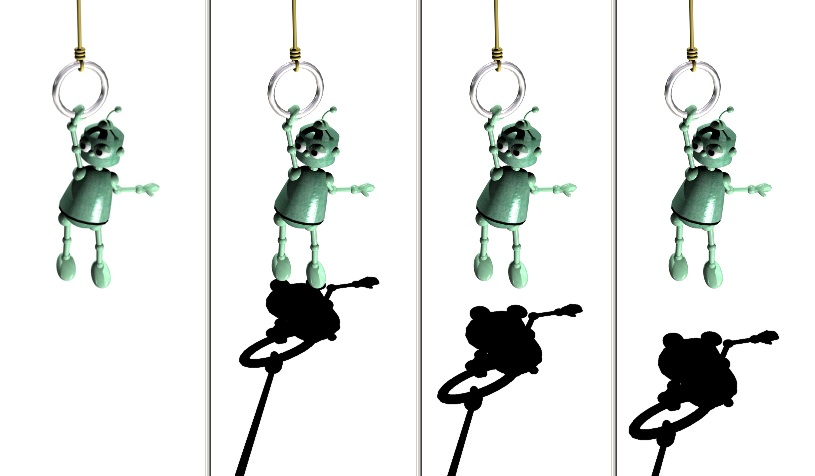
\includegraphics[scale=0.25]{images/relativePosition.jpg}
\centering
\captionsource{L'importance des ombres en image }{http://maverick.inria.fr/Research/RealTimeShadows/importance.html}
\end{figure}

\chapter{Etat de l'art}

Au fil du temps, différents types d'algorithmes permettant de générer ces ombres ont été présentés dans la littérature scientifique. La littérature scientifique distingue donc deux grandes catégories : 
\begin{itemize}
\item les \textit{Hard Shadow},
\item les \textit{Soft Shadow}.
\end{itemize}
Les ombres de type \textit{Hard Shadow} ont été moins considérés ici car elles sont moins réalistes. En effet, ces ombres sont uniformément noires et ne représentent que l'ombre générée par un point lumineux. D'un autre côté, les ombres de type \textit{Soft Shadow} sont beaucoup plus réalistes et sont celles qui sont les plus utilisées. Les algorithmes permettant de faire des ombres de type Soft Shadow seront donc ceux qui seront le plus étudiés ici.

Il existe plusieurs types de \textit{Soft Shadow algorithms}, les principaux sont ceux de:
\begin{itemize}
\item{\textit{Ray tracing}}
\item{\textit{Shadow mapping}}
\item{\textit{Shadow volume}}
\end{itemize}

Ce sont ces trois types d'algorithmes qui ont été étudiés et mis en applications dans ce projet.

\section{Ray tracing}


L'algorithme de \textit{Ray tracing} a été présenté pour la première fois en 1968 par Arthur Appel\cite{appel1968some} sous le nom de \textit{Ray casting}. Il a ensuite été continué, sous le nom de \textit{Ray tracing} cette fois, en 1978 par Whitted \cite{whitted1978scan}, qui y a rajouté la réflexion et la réfraction de la lumière. 
Cet algorithme consiste à tracer un rayon depuis le point de vue jusque chaque pixel créant une \textit{ray surface}. La surface la plus proche du point de vue sera donc celle qui sera visible. A partir de chaque pixel, il faudra ensuite relier la source lumineuse. Si ce rayon a une intersection avec un quelconque objet, ce pixel sera dans l'ombre. Ceci n'est évidemment pas optimal puisqu'il nécessite un calcul pour chaque pixel de la scène.

\section{Shadow volume}


L'algorithme de \textit{Shadow Volume} a été introduit par Crow \cite{crow1977shadow}. Il a ensuite été implémenté grâce à l'accélération  matérielle\cite{fuchs1986fast} mais n'a été que peu utilisé jusqu'à la proposition de Tim Heidmann d'accélérer matériellement cet algorithme sur du matériel accessible au grand public. Cette logique a donné naissance à l'algorithme de \textit{z-pass}\cite{heidmann1991real}. 
\\

La méthode de \textit{z-pass} consiste à premièrement initialiser un \textit{stencil buffer} à zéro et un \textit{depth buffer} avec les valeurs de profondeurs des objets visibles pour ensuite rastérisater les côtés des \textit{shadow volumes}. Pour chaque partie de \textit{shadow volume}, il s'agit ensuite d'incrémenter le pixel du \textit{stencil buffer} correspondant si la face à une normale dans le sens inverse (on rentre alors dans le \textit{shadow volume}) et décrémenté lorsque l'on en ressort. Le \textit{shadow count} représentera alors le niveau d'ombre dans lequel est plongé le point fixé et l'absence d'ombre si celui-ci est égal à 0.\cite{surveyofshadowalgorithms} Ce comptage peut être théoriquement réalisé jusqu'à une distance infinie, grâce à une méthode appelée \textit{z-fail} ou \textit{Depth fail}\cite{bilodeau1999real, carmack2000z}.
\\

Les algorithmes de \textit{z-pass} ont néanmoins un défaut dans le cas où l'on place l'observateur dans l'ombre (dans un ou plusieurs shadow volumes). Ce problème a été en partie résolu par HORNUS et autres\cite{hornus2005zp+}, qui vont proposer d'aligner la vue de la source lumineuse avec celle de l'observateur. Cette technique a été développée en comparant l'algorithme de z-pass, dont ils s'inspirent et qu'ils ont amélioré, avec celui de z-fail. Cette solution n'est pas encore optimale mais à ce jour, aucune autre alternative n'a été proposée.
\\

Dans l'article \cite{lloyd2004cc}, les auteurs présentent une nouvelle technique qui utilise le \textit{Culling and Clamping (CC)} permettant d'éviter de générer des \textit{shadow volumes} qui sont eux-même dans l'ombre ou qui n'interviennent pas dans l'image finale, ce qui a pour but d'améliorer les performances et donc d'accélérer la génération des ombres dans une scène.
\\

Aila et Akenine-Molle font remarquer en 2004 \cite{aila2004hierarchical} que les performances de génération des ombres sont inversément proportionnelles à la taille des \textit{shadow volumes}. Pour remédier à cela, ils proposent un nouvel algorithme visant à réduire le temps de rastérisation. Cet algorithme est composé de deux étapes. La première étape consiste à trouver des zones de 8x8 pixels dont les bords sont soit compl\^etement dans l'ombre soit compl\^etement illuminés. La seconde étape verra s'effectuer une génération pixel par pixel de l'ombre des pixels se trouvant aux bords de l'ombre.
\\

En 2004, Chan et Durand\cite{chan2004efficient} utilisèrent une technique utilisant à la fois un algorithme de \textit{shadow mapping} et un algorithme de \textit{shadow volume}. Le premier est d'abord utilisé pour créer une \textit{hard shadow} et obtenir la silhouette de l'ombre. L'algorithme de \textit{shadow volume} est ensuite utilisé pour généré une ombre correcte (\textit{soft shadow}) à partir de cette silhouette.


\section{Shadow mapping}

L'algorithme de \textit{Shadow Mapping} a, quant à lui, été introduit par Lance Williams \cite{williams1978casting}.
\\

Le principe des \textit{Shadow Mapping Algorithm} est de dresser dans un premier temps une carte de disparité (\textit{depth map/image}) de la scène, comme vue depuis la source de lumière. Pour chaque \textit{texel}, la profondeur de l'objet le plus proche de la source lumineuse sera stockée. Cet algorithme n'est pas optimal et la technique du \textit{Percentage closer filtering}\cite{reeves1987rendering,fernando2005percentage} résoud un problème d'aliasing présent.
\\

Dans le début des années 2000, plusieurs algorithmes utilisant un \textit{filtering} furent présentés. Celui-ci permet d'utiliser une shadow map de basse résolution tout en présentant des résultats convaincants. En 2005, Donelly et Lauritzen \cite{donnelly2006variance} proposent un algorithme utilisant la variance de la distribution des profondeurs, visant à réduire fortement l'aliasing habituellement présent dans les algorithme de \textit{shadow mapping} basiques tout en nécessitant peu de stockages et de calculs supplémentaires. En 2008, un nouvel algorithme est présenté\cite{annen2008exponential}, proposant une autre méthode pour réduire l'aliasing mais avec une technique encore plus efficace et produisant moins d'artefacts graphiques. 
\\

Cependant, l'utilisation de \textit{shadow map} de basse résolution entraine un flou forcé, empêchant la création d'ombres nettes. D'autres algorithmes ont été proposés pour améliorer la précision sans demander de ressources trop énormes. 
\\

Les premiers sont les algorithmes appelés \textit{Perspective Shadow Map}\cite{wimmer2004light,stamminger2002perspective,lloyd2008logarithmic} utilisent le \textit{warping}, qui permet d'avoir de bons résultats mais dégénerent en \textit{shadow map} ordinaire.
\\

Les seconds utilisent le \textit{Partitioning}. Cette approche permet de diviser le frustum de vue et d'utiliser une \textit{shadow map} pour chaque sous-frustum. Cependant, pour être le plus précis possible, cette technique requiert un grand nombre de subdivisions, ce qui affecte les performances.
\\

Un des seuls algorithmes qui présente une précision au pixel près et qui présente des bonnes performances pour le temps réel est celui qui a été présenté par Sintorn et Assarsson\cite{sintorn2009hair}. Celui-ci se focalise sur les ombres de la pilosité, qui nécessite de la précision et obtient pourtant des résultats corrects.
\\

L'algorithme GEARS\cite{wang2014gears} rajoute un élément pris en compte, le dynamisme de la scène illuminée ainsi que celle de la lumière tout en gardant des excellentes performances.


\chapter{Méthodes implémentées}
\todo{parler plus de l'environnement, genre plusieurs lampes et tout}

Dans ce chapitre, nous allons décrire les différents algorithmes implémentés et l'environnement dans lequel ils ont été testé.

\section{Choix de l'environnement de test}

L'environnement est important. En effet, c'est sur celui ci que les différents algorithmes vont s'appliquer. En choisissant le m\^eme environnement pour tous les algorithmes nous pourront comparé leur performance en utilisant différentes \textit{metrics}.

\subsection{La 3D}

OpenGL s'est imposé comme l'API 3D de choix étant donné sa spécification ouverte, ses fonctions bas niveau et sa disponibilité sur un grand nombre de plateformes.
Nous avons utilisé OpenGL pour créer des scènes 3D, animer une/des caméra(s) et une/des source(s) de lumière mais également pour générer des ombres avec les algorithmes retenus.

Nous avons utilisé dans la mesure du possible un maximum les fonctions modernes d'OpenGl majoritairement présente dans les jeux et animations d'aujourd'hui. Le code propre a la 3D sera donc des shaders.

Nous avons aussi choisi de ne pas utilisé de moteur de rendu 3D pour car utiliser à la place directement le langage de bas niveau OpenGL permet d'avoir une approche plus fine et de maitriser plus de paramètre. En outre, cela permet de mieux comprendre le fonctionnement de la 3D et cette approche ne masque pas les opérations qui sont faites ce qui facilite a la comparaison des algorithmes.

\subsection{Langages et bibliothèques utilisés}

Les langages utilisés influencent les performances globales des algorithmes et du programme de test. Cependant, si pour chaque algorithme on utilise le m\^eme langage, il sera toujours possible de les comparer. Nos choix ont donc été basés sur l'interopérabilité du langage de programmation et de OpenGL. Ils sont les suivants :

\begin{itemize}
\item{Nous avons utilisé Python 2.7 comme langage de programmation car il permet un développement rapide et possède des bindings vers les bibliothèques OpenGL, OpenCL, numPy etc... écrites en C/C++. Il permet donc d'allier la rapidité d'écriture des langages de scripts à la rapidité d'exécution des langages compilés. Nous avons aussi utilisé des package du Python Package Index pour nous faciliter la t\^ache.}

\item{Nous avons utilisé pyQt comme librairie qui s'interfacera avec la célèbre bibliothèque Qt 5. Nous avons utilisé cette interface graphique étant donnée sa facilité d'utilisation et son caractère complet. De plus nous avions pour la plupart déjà utilisée cette dernière durant notre cursus.}

\item{Nous comptions utiliser OpenCL pour profiter de puissance de calcul des cartes graphiques modernes. Nous ne l'avons finalement pas utilisé car nous nous sommes redirigés vers la puissance de calcul de numpy associée avec quelques parties d'implémentation en C++}

\item{Nous avons enfin utilisé vispy, librairie de visualisation 3D basée sur OpenGL qui permet d'utiliser les avantages d'OpenGL moderne et d'utiliser des shaders avec une certaine abstraction. Ceci permet d'effectuer les calculs de rendu graphique directement sur le GPU, ce qui accroit la vitesse d'exécution et donc les performances.
}
\end{itemize}

\subsection{Scènes présentées}

Plusieurs scènes ont été utilisées pour présenter et mettre en application les différents algorithmes. 

\subsubsection{Création des scènes}
Il est intéressant de pouvoir placer des modèles en hauteur, à différents endroits. Ceci permet de démontrer que lorsque les ombres sont absentes, on ne peut percevoir les informations relatives ni à la hauteur, ni au relief.

Pour cela nous avons utiliser deux ressources :

\begin{enumerate}
  \item Des fichiers de configuration de la scène en JSON,
  \item Des modèles 3D au format libre OBJ.
\end{enumerate}

Un dossier prédéfinit contient un certain nombre de fichier JSON qui eux contiennent toutes les informations nécessaires a la création d'une scène. Ils contiennent :

\begin{enumerate}
  \item Le nom de la scène,
  \item Une courte description de la scène,
  \item Quels modèles 3D sont inclus à la scène,
  \item Les algorithmes compatibles avec la scène,
  \item La position de ces modèles 3D.
\end{enumerate}

Les modèle 3D au format OBJ proviennent de site internet proposant des modèles libres de droit et sont très divers de manière à pouvoir réaliser beaucoup de test différents : vélo, fractal de menger, mario et luigi, arbres, ...

\subsubsection{Lumières}

Les lumières ont bien évidemment une importance capitale dans notre environnement de test.

Nous n'avons implémenté que des lumières ponctuelles de couleur blanche. Nous pouvons par contre en mettre autant que souhaité et les mettre à la position de notre choix. De plus il est possible via un sélectionneur dans la barre d'outils de les déplacer en temps réel. Cela permet de tester les positions critiques des ombres ou des glitch pourrait apparaitre.


\subsubsection{Animations}

Pour rendre le programme plus interactif et pour pouvoir mieux observé les ombres, nous avons implémenté deux animations différentes.

Une première qui consiste a faire tourner de manière régulière la caméra autour du centre de la scène.

une deuxième qui consiste a faire tourner la lampe sélectionner dans la barre d'outils.

\subsection{Metrics utilisé}

Pour mesurer la performance d'un algorithme nous avons utilisé différentes mesures.
\subsubsection{Image par seconde}
Le nombre d'image par seconde ou Frame par second (FPS) en anglais est une mesure indiquant le nombre d'image affiché par seconde sur un écran. Plus ce nombre est élevé plus l'animation semble fluide.
La méthode de calcul utilisé est la suivante :

$nombre de fps = \frac{1 seconde}{Temps  nécessaire pour générer une frame}$


Pour obtenir un résultat stable, une moyenne est faite sur un échantillon d'une durée de 1 seconde.

\subsubsection{CPU}
Une librairie python permet de mesurer le pourcentage d'utilisation du processeur en par le programme courant. Une haute utilisation indique un algorithme peu performant.
\subsubsection{Mémoire}

Une librairie python permet de mesurer le nombre de megabytes de mémoire vive utilisé par le programme courant. Une haute utilisation indique un algorithme peu performant.

\section{Algorithmes implémentés} 

\subsection{Shadow volume}

\begin{figure}[H]
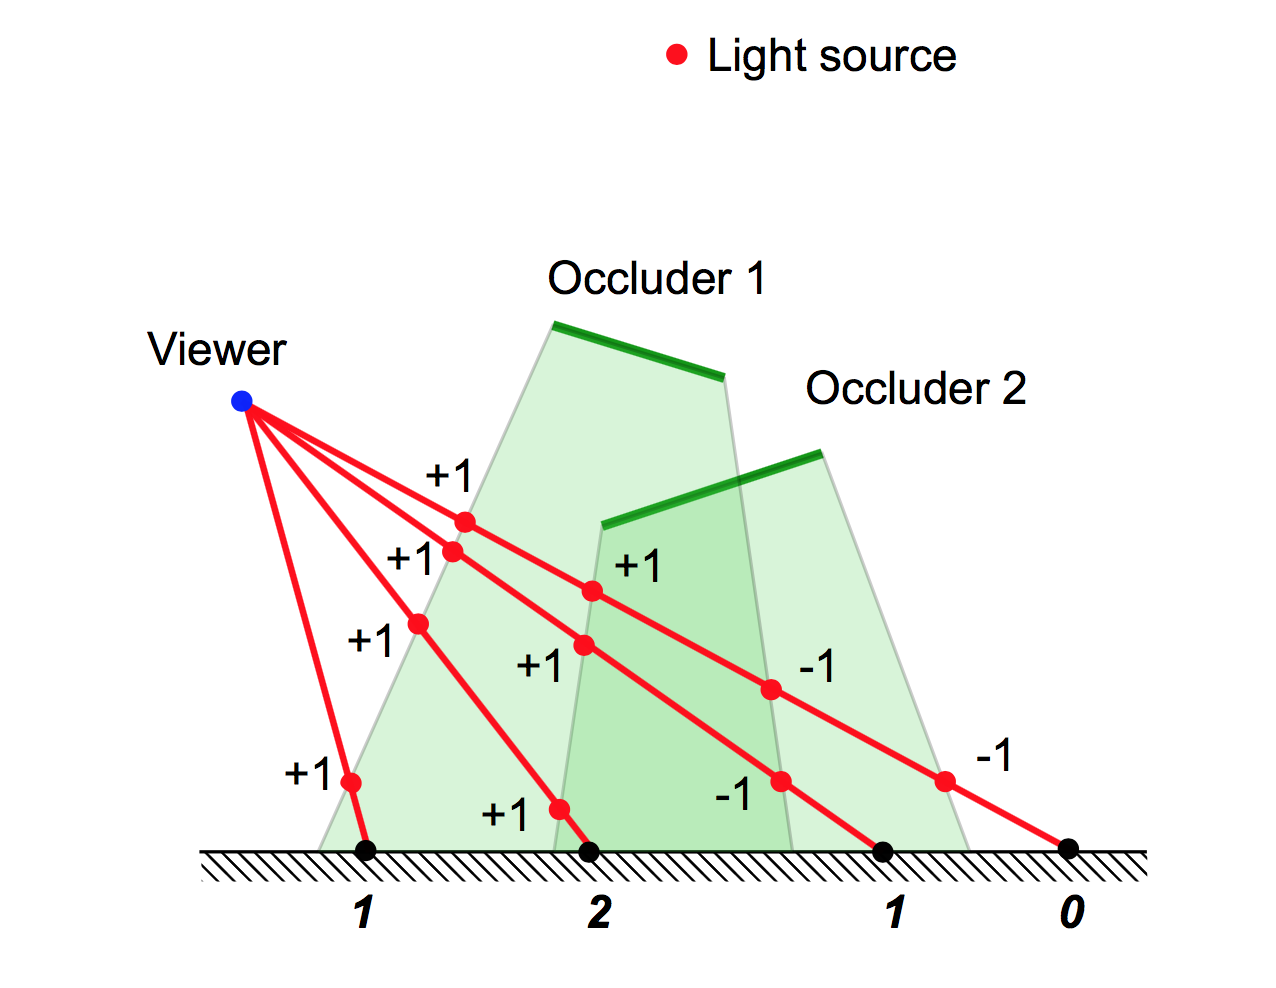
\includegraphics[scale=0.5]{images/shadow_volume.png}
\centering
\captionsource{Shadown volume}{https://hal.inria.fr/inria-00281388}
\end{figure}
L'algorithme de shadow volume peut être divisé en deux étapes.

Tout d'abord, il s'agit de trouver les contours de chaque objet chargé dans la scène depuis le point de vue de la lumière. 
Puisque le point de vue se trouve à la position de la lumière, les contours à trouver sont toutes les arêtes communes à un triangle se trouvant dans la lumière et un triangle se trouvant dans l'ombre. 
L'algorithme fonctionne en ajoutant les are\^tes des triangles situés dans l'ombre dans une liste et en les enlevant de la liste si ils sont déjà dedans.
De cette manière, seules les arêtes qui ne sont pas communes à deux triangles dans l'ombre (donc qui sont communes à un triangle dans l'ombre et un dans la lumière) sont conservées.
Pour déterminer si un triangle est dans l'ombre ou la lumière, on calcule le vecteur normal de ce triangle et on fait le produit scalaire de ce vecteur avec le vecteur de direction de la lumière. Si le résultat est positif, le triangle est dirigé dans le même sens que la lumière et donc se trouve sur le co\^té opposé à la lumière.
Une fois que les are\^tes définissant les contours sont déterminées, on les projette à l'infini dans la direction opposée à la lumière ce qui crée une homothétie du contour. Le contour de l'objet et son homothétie délimitent alors un volume, appelé shadow volume ou volume d'ombre. 
Nous avons commencé par implémenter cette étape en Python avant de nous rendre compte que la puissance de calcul nécessaire était trop grande.
Cette étape est donc implémentée dans une fonction en C++ appelée depuis le code Python.

Une fois que ces volumes sont générés, il suffit de déterminer quels objets ou parties d'objets se situent dans un ou plusieurs volumes, et de ce fait, dans l'ombre. 
Pour ce faire, le rendu de la scène est effectué une première fois sans la lumière pour dessiner la scène dans l'ombre.
Ensuite le rendu de la scène est effectué deux fois en activant le stencil test dans OpenGL et en désactivant l'écriture sur le color buffer et le depth buffer, de manière à ne pas modifier l'image affichée. La première fois, on incrémente la valeur du stencil buffer chaque fois que l'on rentre dans un shadow volume (en activant le back-face culling). La deuxième fois on le décrémente chaque fois que l'on en sort (avec le front-face culling). Pour chaque pixel de la scène, on obtiendra alors une valeur valant soit zéro pour un point situé dans la lumière soit une valeur plus grande représentant l'intensité de l'ombre.
Un nouveau rendu est alors effectué avec la lumière uniquement aux endroits où le stencil buffer est égal à zéro.


\subsection{Shadow mapping}

\begin{figure}[H]
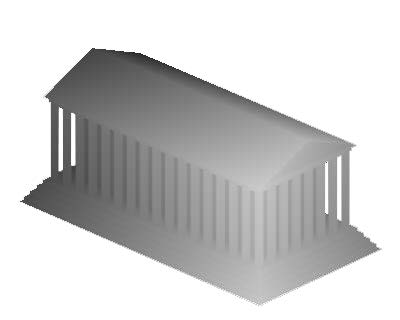
\includegraphics[scale=0.5]{images/shadow_map.jpg}
\centering
\captionsource{Shadown mapping}{wikipedia.org}
\end{figure}

L'algorithme de shadow mapping se déroule également en deux étapes.

La première étape consiste à générer une shadow map d'une résolution choisie. Une shadow map est une représentation depuis le point de vue de lumière de la profondeur de chaque point de la scène. Pour ce faire, OpenGL offre la structure d'un depth buffer, permettant de calculer la profondeur de chaque pixel visible depuis la lumière en effectuant le rendu.

Dans la seconde étape, on effectue le rendu de la scène depuis la caméra. On considère pour chaque pixel sa distance à la lumière par rapport à la profondeur au même endroit dans la shadow map. Si la première est plus grande que la seconde, alors ce pixel est dans l'ombre et sa couleur est assombrie.
On simule également la réflexion spéculaire en prenant en compte le vecteur normal de chaque pixel par rapport au vecteur direction de la lumière. Plus un pixel est tourné vers la lumière, plus sa couleur est illuminée.

Si la scène considérée contient plusieurs sources lumineuses, le principe d'implémentation reste identique. Il suffit alors de réaliser différentes shadow map, chacune avec le point de vue d'une lumière. Ces différentes ombres sont superposées en assombrissant un pixel proportionnellement au nombre d'ombres dans lequel il se trouve.

Un apport a été effectué pour approcher d'une soft shadow en utilisant une méthode de dispersion des points d'ombre à l'aide d'un disque de Poisson, ce qui floute les contours de l'ombre et ajoute au réalisme.


\subsection{Ray tracing}	

Le ray tracing consiste à tracer un segment de droite depuis le point de vue de l'observateur jusque chaque pixel de la scène. Ce segment de droite simule un rayon de lumière en sens inverse. A partir de ce pixel, on lance un rayon vers l'ensemble des sources lumineuses de manière à déterminer sa luminosité. En effet si un rayon rencontre un autre objet avant de rencontrer une source lumineuse, cela signifie que cet objet est dans l'ombre par rapport à cette source lumineuse.

On peut noter que cette technique est fonctionne a rebours de la réalité physique ou le rayon lumineux par de la lumière pour arriver à l'oeil de l'observateur. Elle permet donc une très bonne simulation du comportement de la lumière mais n'est pas applicable en temps réel. C'est pourquoi la scène où nous avons implémenté le ray tracing n'est pas interactive.


\begin{figure}[H]
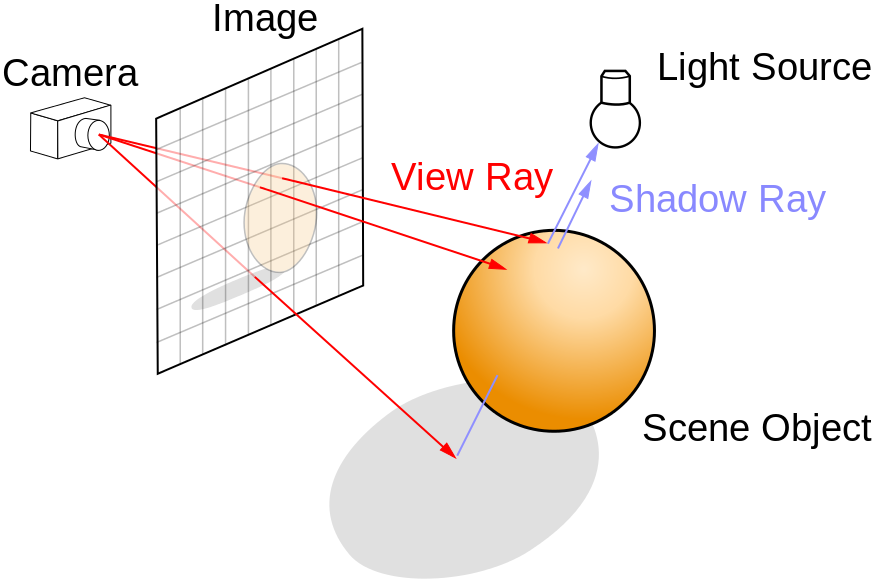
\includegraphics[scale=0.5]{images/ray_tracing.png}
\centering
\captionsource{Ray Tracing}{wikipedia.org}
\end{figure}


\chapter{Résultats expérimentaux}

\section{Les ombres sont indispensables}

Dans notre environnement de test, nous avions implémenté deux mises en scènes, une sans ombre et une avec ombre.

Il a été remarqué que l'absence d'ombres privait non seulement de réalisme les scènes considérées mais également d'informations quant au relief et à la position des objets et des personnages que présente la scène. En effet si on prend par exemple la scène ou l'on voit un personnage le fait de ne pas avoir d'ombre semble montré au spectateur que le personnage est un dessin 2D sans relief peu esthétique.

Après avoir ajouté uniquement l'ombre que les objets et personnages créent sur eux-même, l'information quant au relief est apportée mais pas celle de position. Gr\^ace a cela, on a pu confirmer que c'est donc bien l'ombre d'un élément de la scène sur l'autre et non sur lui-même qui permet à l'observateur de déterminer sa position relative.

\section{Les différents types d'ombre}

D'après nos résultats subjectif, les algorithmes hard shadow

\section{Résultats individuels}

\subsection{Shadow volume}
\todo{On peut dire que on a a du mal, qu'on a du faire du c++ et tout voila}
\todo{pourquoi c'est lent en python, pourquoi ca ne marche tjs pas (opengl...), résultats pour le moment}


\subsection{Shadow mapping}

Comme prévu, cet algorithme est le plus efficace des trois algorithmes considérés. Le résultat obtenu obtient un nombre de \textit{fps} plus que correct. Le réalisme offert dépend en grande partie de la résolution imposée de la shadow map. Une grande shadow map implique une grande précision mais également un plus grand nombre de calculs à réaliser. Cette approche apporte donc une ombre correcte et donc l'apport d'information qui en dépend. La résolution de la shadow map, influençant la précision de l'ombre peut toutefois être changée, pour offrir une ombre plus ou moins pixelisée. Puisque la shadow map est calculée du point de vue de la lumière, plus celle-ci est loin de la scène, plus la résolution nécessaire pour obtenir une bonne précision est grande.
Les ombres sont crénelées à cause de la résolution limitée de la shadow map. Pour résoudre ce problème, on peut ajouter un biais lors du sampling dans la shadow map mais si ce biais devient trop grand, les ombres "flottent".
De la même manière on peut ajouter du réalisme en modifiant la répartition du disque de Poisson mais en augmentant la répartition de trop, on voit apparaître des nuages de points dans l'ombre.

\todo{PLUS DE DETAILS ICI VOILA VOILA}

\subsection{Ray tracing}hat do ? on a rien =/

Cet algorithme étant le plus gourmand en ressources de calculs, il n'a été implémenté qu'en version non-interactive et la scène qui l'implémente ne contient qu'un mouvement continu sur 2 objets, n'appliquant pas l'ombre de l'un sur l'autre, de sorte à réduire les calculs nécessaire et avoir une scène qui pourra être utilisée pour l'observation de la qualité de l'ombre générée. Celle-ci est parfaite, étant donné le fait que l'algorithme consière chaque pixel de la scène indépendament. L'ombre va donc être appliquée sur chaque pixel un à un, et cet algorithme va donc offrir une précision au pixel près. Le ray tracing offre donc un excellent rendu d'ombre mais nécessite du matériel extrêmement puissant ou une réduction volontaire du nombre de calculs.


\section{Comparaison des algorithmes entre eux}


\begin{table}[h]
\centering
\begin{tabular}{|c|c|c|c|l}
\cline{1-4}
 & FPS  & CPU & Mémoire  &  \\ \cline{1-4}
 Aucune ombre& 400 & 20\%  & 3,2\%  &  \\ \cline{1-4}
 Auto ombre& 225 & 28\%  & 3,2\%  &  \\ \cline{1-4}
 Ray tracing& ? & ?  & ?  &  \\ \cline{1-4}
 Shadow mapping& 250  & 30\%  & 3,2\%  &  \\ \cline{1-4}
 Shadow volume& 120  & 20\%  & 3,2\%  &  \\ \cline{1-4}
\end{tabular}
\end{table}

Il ne nous est pas possible de comparer le Ray Tracing car nous n'avons pas réussi à faire en sorte qu'il crée l'ombre en temps réel dans notre environement de test. Ceci n'est pas étonnant sachant qu'il fait un très grand nombre de calcul.Cependant, il permet donc d'obtenir les meilleurs résultats lorsque les performances ne sont pas un facteur limitant, comme par exemple pour des animations qui ne sont pas en temps réels, ou même des images fixes pour des logiciels d'édition d'image.

Moins précis que ce dernier mais également plus performant et plus adapté aux représentations en temps réel, l'algorithme de Shadow Volume offre quant à lui une excellent rapport entre performances et précision. 

\todo{Ceci est une discussion par un resultat imho}C'est pour cette raison que cet algorithme est utilisé dans des logiciels d'animation nécéssitant du temps réel, comme le logiciel utilisé chez Pixar, \textit{PhotoRealistic RenderMan}.

Le plus performant mais également le moins précis des trois algorithmes que nous avons ici considéré est le shadow mapping. Celui-ci est toutefois le seul a offrir plusieurs niveaux de précision en fonction de la résolution qui est choisie pour la shadow map.


\chapter{Discussion}

\section{Cas d'utilisation des algorithmes}
\subsection{Ray Tracing}
\subsection{Shadow mapping}
\subsection{Shadow volume}

\section{Alternatives}

\section{Approches utilisées dans l'industrie}


\chapter{Conclusion et perspectives}

Conformément aux informations qui avaient été extraites de la littérature scientifiques , les ombres apportent des informations quant à la position des différents éléments d'une scène 3D, ainsi qu'un apport de réalisme nécessaire aux animations et aux jeux vidéos. Sans ombre, il n'y a pas non plus de perception de relief pour une scène 3D. Le relief est pourtant crucial dans une animation ou un jeu vidéo car sans lui, la 3D ne sera pas perçue. 

Les deux types d'ombres ont été considérés dans cette étude., les hard shadows comme les soft shadows. Les premieres sont les ombres qui sont celles dues à une seule source lumineuse ponctuelle. Elles sont donc quasi inexistantes dans la nature. En comparaison avec celles-ci, les soft shadows, ombres diffuses, sont abondamment plus réalistes. En effet, elles sont le résultat d'éléments placés dans un environnement illuminé de force source lumineuses ponctuelles, comme retrouvés dans la nature.
Au fil du temps, les sociétés d'animation et de développement de jeux vidéos se sont tournés des hard shadows vers les soft shadows lorsque le matériel le permettait, dans le but d'obtenir une hausse de réalisme.

Nous avons ici implémenté et comparé 3 types



\bibliographystyle{apalike}

\bibliography{mybiblio.bib}
\addcontentsline{toc}{chapter}{Bibliographie}

\end{document}